\section{Radioactivity: Detection methods}

%\frame{\tableofcontents[currentsection]}

\begin{frame}{Thinking over \ldots}

\begin{exampleblock}{Key questions}

\begin{itemize}
	\item What do we need to measure? 
	\item How can we do the measurements?
	\item Which parameters are important ? 
\end{itemize}

\end{exampleblock}


\pause

\begin{alertblock}{Boundary conditions}

\begin{itemize}
	\item Facilities
 	\item Staff’s training
 	\item Accuracy and precision
 	\item Deadline for results
 	\item Our budget 
\end{itemize}

\end{alertblock}

\end{frame}


\begin{frame}{Available techniques}

\begin{itemize}
	\item Alpha spectrometry
 	\item Liquid Scintillation counting (LSC)
 	\item Gross alpha / beta
 	\item Gamma spectrometry
 	\item Others (i.e., ICP-MS and others)
\end{itemize}

\centering \arrowdown

\vskip0.5cm \centering \alert{{\large Advantages and disadvantages}}

\end{frame}

\begin{frame}[allowframebreaks]{Alpha spectrometry}

\begin{exampleblock}{Characteristics}

\begin{itemize}
	\item High resolution surface barrier detectors
  \item Low Detection limits possible in a reasonable measurement time
  \item Good definition of peaks
 \item Possible to measure a lot of natural radionuclides (uranium and thorium series)
\item  Calibration is easy, no problem with geometries
\end{itemize}

\end{exampleblock}

\begin{alertblock}{Problems}

\begin{itemize}
	\item Radiochemistry (separation)
 \item Adsorption (i.e., radium isotopes)
\item  Chemical interferences (barium) 
 \item Interferences in spectrum
 \item Costly technique
\end{itemize}

\end{alertblock}

%\end{frame}
%
%\begin{frame}{Alpha spectrometry}

\centering
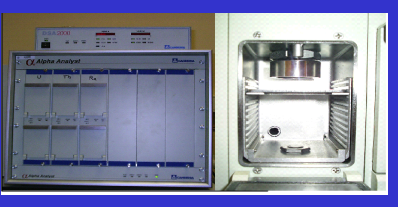
\includegraphics[scale=0.8]{figures/alpha_device.png}

\end{frame}

\begin{frame}[allowframebreaks]{LIQUID SCINTILLATION COUNTING }

\begin{exampleblock}{Characteristics}

\begin{itemize}
	\item $\alpha$/$\beta$ Discrimation
 \item Low detection limits can be reached
 \item Not long measurement times
 \item Possibility to handle a large number of samples  
\end{itemize}

\end{exampleblock}

\begin{alertblock}{Problems}

\begin{itemize}
	\item Problems with spillover
 \item Correct Set up of the LSC counter can be difficult
 \item When measuring $^{226}$Ra seqular eqilibrium with $^{222}$Rn is needed: time consuming
 \item LSC counter is very expensive
\end{itemize}

\end{alertblock}

%\end{frame}
%
%\begin{frame}{LIQUID SCINTILLATION COUNTING }

\centering
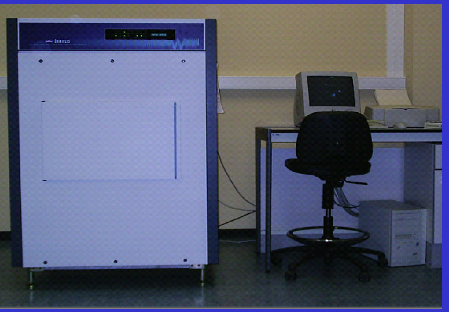
\includegraphics[scale=0.5]{figures/quantulus.png}

\end{frame}

\begin{frame}[allowframebreaks]{Gamma spectrometry}

\begin{exampleblock}{Characteristics}

\begin{itemize}
	\item Instrumentation (HPGe) available in most of labs 
 \item No radiochemistry is needed
\item  Pretreatment of the sample is very simple
 \item A large number of radionuclides can be measured
 \item Detection limits acceptable for environmental determinations
\end{itemize}

\end{exampleblock}

\begin{alertblock}{Problems}

\begin{itemize}
	\item Each geometry needs different efficiency calibration
 \item Very dependent on density of sample
 \item Time consuming (several days in some cases)
 \item Maintenance of detector is critical (refrigeration)
 \item Monitoring of background levels is necessary
\end{itemize}

\end{alertblock}

%\end{frame}
%
%\begin{frame}{Gamma spectrometry}

\centering
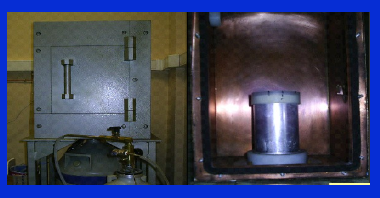
\includegraphics[scale=0.7]{figures/hpgelaruc.png}

\end{frame}

\begin{frame}{Short intro to gamma spectrometry}


\begin{figure}
\centering
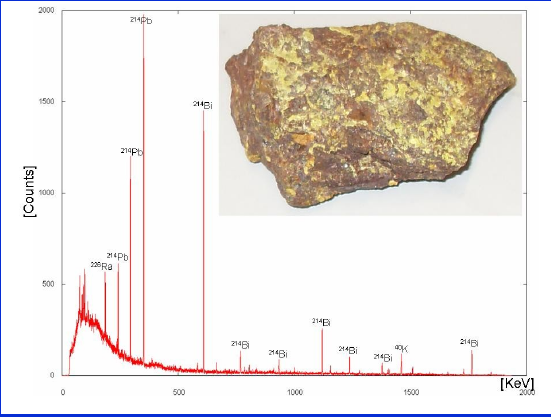
\includegraphics[scale=0.4]{figures/pechblenda.png}
\caption*{The gamma-ray spectrum of natural uranium, showing about a dozen discrete lines superimposed on a smooth continuum, allows the identification the nuclides $^{226}$Ra, $^{214}$Pb, and$^{214}$Bi of the uranium decay chain. (\emph{Credit: wikipedia})}
\end{figure}


\end{frame}

\begin{frame}[allowframebreaks]{Short intro to gamma spectrometry}


\begin{exampleblock}{Gammna decay: Photon’s emission by a nucleus when reaching steady state of energy}

\begin{itemize}
	\item Gamma line is the fingerprint of a radionuclide 
	\item One radionuclide can have several gamma lines with different probabilities and different energies 
	\item X Rays and Gamma Rays (with different energies) 
	\item Gamma rays = Nucleus 
	\item X Rays = Atomic crust
\end{itemize}

\end{exampleblock}


\begin{exampleblock}{INTERACTION OF RADIATION WITH MATTER}


\begin{itemize}
\item Charged particles produce a signal within a detector by ionization and excitation of the detector material directly. 
\item Gamma photons are uncharged and consequently cannot do this 
\item Gamma-ray detection depends upon other types of interaction which transfer the gamma-ray energy to electrons within the detector material 
\end{itemize}

\end{exampleblock}

\begin{exampleblock}{INTERACTION OF RADIATION WITH MATTER}


\begin{itemize}
\item Excited electrons charge and lose their energy by ionization and excitation of the atoms of the detector medium, giving rise to many electron–hole pairs 
\item The absorption coefficient for gamma radiation in gases is low and all practical gamma ray detectors depend upon interaction with a solid 
\item The electron–hole pairs can be collected and presented as an electrical signal.
\end{itemize}

\end{exampleblock}

\end{frame}

\begingroup

\setbeamercolor{normal text}{fg=\cnDarkGrey,bg=\cnLightGreen}
\begin{frame}{How do radiation and matter interact?}

\pause

\setbeamercolor{boxsthlmBlue}{bg=\cnBlue,fg=white}\begin{beamercolorbox}[wd=\linewidth,ht=5ex,dp=3ex]{boxsthlmBlue}\centering PHOTOELECTRIC EFFECT\end{beamercolorbox}

\pause

\setbeamercolor{boxsthlmBlue}{bg=\cnBlue,fg=white}\begin{beamercolorbox}[wd=\linewidth,ht=5ex,dp=3ex]{boxsthlmBlue}\centering COMPTON EFFECT\end{beamercolorbox}

\pause

\setbeamercolor{boxsthlmBlue}{bg=\cnBlue,fg=white}\begin{beamercolorbox}[wd=\linewidth,ht=5ex,dp=3ex]{boxsthlmBlue}\centering PAIR PRODUCTION \end{beamercolorbox}


\end{frame}
\endgroup

\begin{frame}{PHOTOELECTRIC EFFECT}

\vskip0.3cm
\alert{The photon interacts with the atom and gives ALL its energy to one electron: one part of the energy is used as kinetic energy and the rest is used to remove electron from the atom}

\vskip0.5cm
\centering
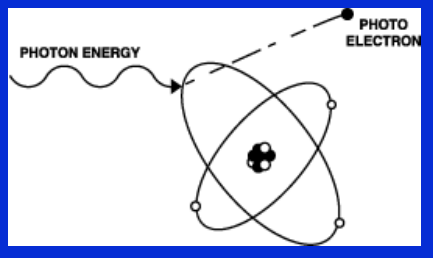
\includegraphics[scale=0.5]{figures/photoelectriceffect.png}

\end{frame}

\begin{frame}{COMPTON EFFECT}

\vskip0.3cm
\begin{exampleblock}{Characteristics}

\begin{itemize}
\item ``Elastic collision'': pool balls 
\item Main interaction of gamma rays 
\item The photon collides with electron and hands over part of its energy to it. The angle through which the photon is scattered, the energy handed on to the electron, and energy lost by the photon are interconnected
\end{itemize}

\end{exampleblock}


\centering
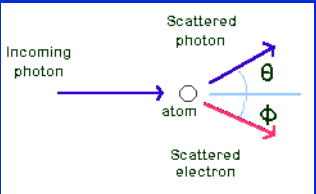
\includegraphics[scale=0.4]{figures/comptoneffect.png}

\end{frame}


\begin{frame}{PAIR PRODUCTION}

\vskip0.3cm
\begin{exampleblock}{Characteristics}

\begin{itemize}
\item When the photon with energy in excess of 1.02 MeV passes close to the nucleus of an atom, the photon disappears, and a positron (e$^{+}$) and an electron (e$^{-}$) appear 
\item Annihilation reaction: positron interacts with electrons and creates 2 annihilation photons each of 0.51 MeV
\end{itemize}

\end{exampleblock}

\centering
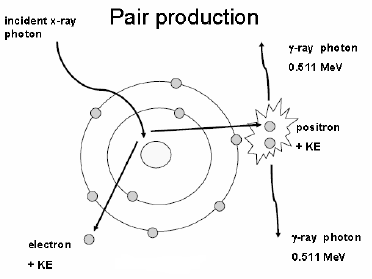
\includegraphics[scale=0.5]{figures/pairproduction.png}

\end{frame}

\begin{frame}{Interaction radiation and matter}

\begin{exampleblock}{Key facts}

\begin{itemize}
\item Photoelectric interactions are dominant at low energy 
\item Pair production at high energy 
\item Compton scattering being most important in the mid-energy range 
\item In practice, evidence of pair production is only seen within a gamma-ray spectrum when the energy is rather more than 1022 keV
\end{itemize}

\end{exampleblock}

\end{frame}

\begin{frame}[allowframebreaks]{Let's study one spectrum}
\centering
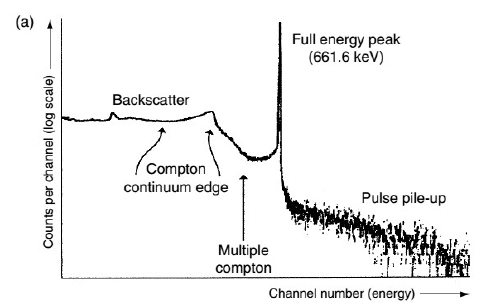
\includegraphics[scale=0.6]{figures/gammaspecexample.png}


\begin{exampleblock}{What can we infere?}

{\small
\begin{itemize}
\item Counts to appear in the spectrum above the full energy peak (apart from the natural background): due to random summing or pile-up, determined by the statistical probability of two gamma-rays being detected at the same time and therefore on the sample count rate 
\item The most troublesome photoelectric interactions will be those with the shielding, usually lead. There is a significant possibility that this fluorescent X-ray may escape the shielding and that it will be detected by the detector: generation of a number of X-ray peaks in the gamma spectrum in the region 70–85 keV (problems for low energy measurements that may be solved with Cd and Cu) 
\end{itemize}
}
\end{exampleblock}

\begin{exampleblock}{What can we infere?}

{\small
\begin{itemize}
\item The normal geometric arrangement of source–detector shielding means that most gamma-rays are scattered through a large angle by the shielding: backscattering (difficult to solve)
\item Pair production: surroundings of the detector give rise to the annihilation peak at 511 keV in the spectrum. This is caused by the escape of one of the 511 keV photons from the shielding, following annihilation of the pair production positron. The annihilation peak is clearly visible in the spectrum of $^{28}$Al (see Figure) but not in that of $^{137}$Cs \alert{(Why?})
\end{itemize}
}
\end{exampleblock}



\centering
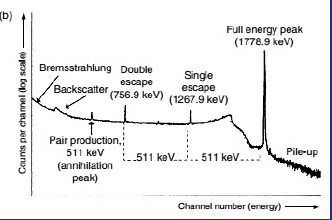
\includegraphics[scale=0.6]{figures/specal28.png}

\end{frame}


\begin{frame}{Practical points gamma detection}


{\small
\begin{itemize}
\item Gamma spectrometry using germanium detectors is the best technique for identifying and quantifying radionuclides. This is due to the very sharply defined and characteristic energies of gamma-rays which are produced by the great majority of radionuclides. 
\item There are a small number of ‘pure beta emitters’, which do not emit gamma radiation. These cannot be identified by gamma spectrometry ($^{3}$H, $^{14}$C, $^{90}$Sr). 
\item X-ray energies will tell you the element present, but not which isotope. 
\item Decay schemes give vital information on whether gammas are in ‘cascade’. This has great significance in true coincidence summing.
\end{itemize}
}


\end{frame}

\begin{frame}{Practical points detection systems}

\setbeamercolor{boxsthlmBlue}{bg=\cnBlue,fg=white}\begin{beamercolorbox}[wd=\linewidth,ht=5ex,dp=3ex]{boxsthlmBlue}\centering Radiation INTERACTS with matter (detector's material)\end{beamercolorbox}


\pause
\centering \arrowdown

\pause
\setbeamercolor{boxsthlmBlue}{bg=\cnBlue,fg=white}\begin{beamercolorbox}[wd=\linewidth,ht=5ex,dp=3ex]{boxsthlmBlue}\centering We must \emph{translate} this interaction into an electrical signal that we are able to measure\end{beamercolorbox}



\end{frame}



\begin{frame}{Ideal properties of gamma spectrometry detector}


{\small
\begin{itemize}
\item Output proportional to gamma-ray energy 
\item good efficiency, i.e. high absorption coefficient, high Z 
\item easy mechanism for collecting the detector signal 
\item good energy resolution 
\item good stability over time, temperature and operating parameters 
\item reasonable cost
\item reasonable size
\end{itemize}
}


\end{frame}

\begin{frame}{Band structure of solids}

\centering
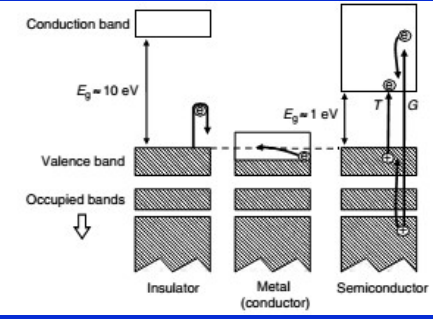
\includegraphics[scale=0.6]{figures/bands.png}

\end{frame}

\begin{frame}{Charge carriers}


{\small
\begin{itemize}
\item The interaction of a gamma-ray with the semiconductor material will produce primary electrons with energies considerably greater than thermal energies 
\item Electric field, carriers will migrate up (electrons) or down (holes) the field gradient. 
\item The number of electron–hole pairs produced, n, will be related directly to the gamma-ray energy absorbed 
\item One important component of the detector resolution is a function of n 
\item Avoid trapping centres which can make difficult mobility of carriers: the detector material must be available, at reasonable cost, with a high purity and as near perfect as possible crystalline state
\end{itemize}
}


\end{frame}

\begin{frame}{Suitable materials?}


{\small
\begin{itemize}
\item To have as large an absorption coefficient as possible (i.e. high atomic number)
\item To provide as many electron–hole pairs as possible per unit energy
\item To allow good electron and hole mobility
\item To be available in high purity as near perfect single crystals
\item To be available in reasonable amounts at reasonable cost.
\end{itemize}
}


\end{frame}

\begin{frame}[allowframebreaks]{Type of HPGe detectors}

\alert{Intrinsic semiconductor: A semiconductor material containing equal numbers of electrons and holes}


{\small
\begin{itemize}
\item acceptor impurities when distributed throughout the semiconductor material give rise to extra energy states just above the valence band, called acceptor states. Germanium with this type of impurity would be called p-type germanium (‘p’ for positive acceptor impurities) 
\item The impurity atom is a donor atom sitting in a donor site, it will introduce donor states just below the conduction band. Germanium with such impurities is n-type germanium (‘n’ for negative donor impurities)
\item The p-type material has an excess of holes and the n-type an excess of electrons.
\end{itemize}
}


\centering
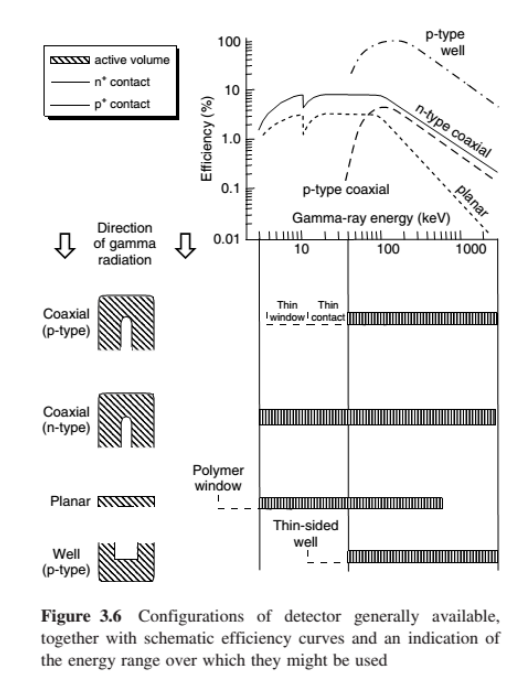
\includegraphics[scale=0.3]{figures/typehpge.png}

\end{frame}

\begin{frame}[allowframebreaks]{HPGe detectors}

\setbeamercolor{boxsthlmBlue}{bg=\cnBlue,fg=white}\begin{beamercolorbox}[wd=\linewidth,ht=10ex,dp=3ex]{boxsthlmBlue}\centering Germanium detectors are operated at low temperature in order to reduce electronic noise and thereby achieve as high a resolution as possible\end{beamercolorbox}

\centering \arrowdown

\setbeamercolor{boxsthlmBlue}{bg=\cnBlue,fg=white}\begin{beamercolorbox}[wd=\linewidth,ht=6ex,dp=3ex]{boxsthlmBlue}\centering The most common means of providing a suitably low temperature is cooling with liquid nitrogen (boiling point 77 K)\end{beamercolorbox}


\begin{figure}
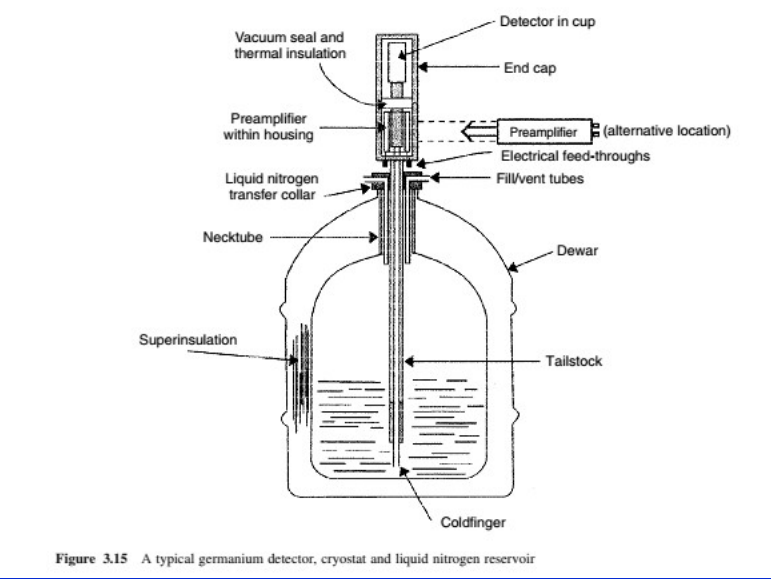
\includegraphics[scale=0.4]{figures/schemehpge.png}
\end{figure}

\end{frame}

\begin{frame}{HPGe detectors: example}
\begin{figure}
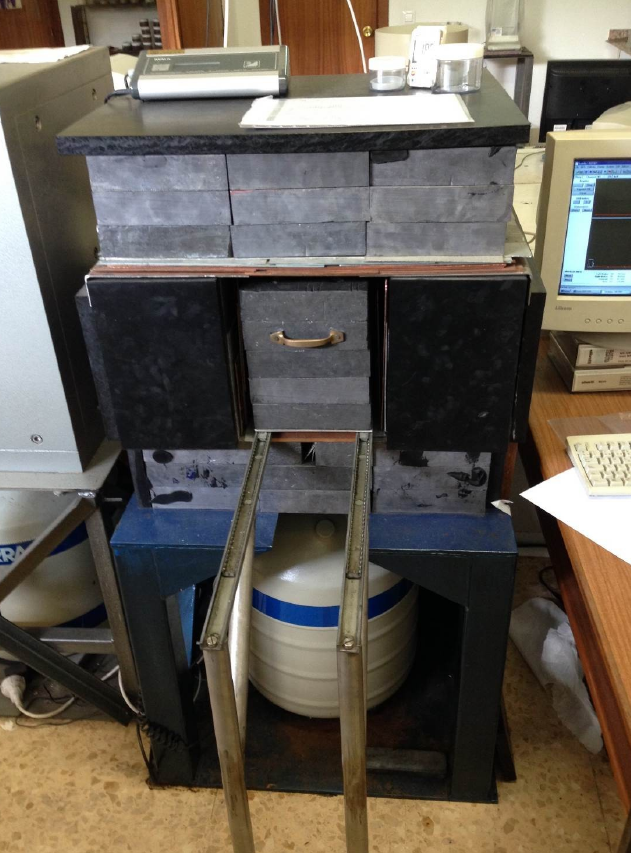
\includegraphics[scale=0.25]{figures/hpgelaruc2.png}
\end{figure}
\end{frame}

\begin{frame}{HPGe detectors: Detection system}


\centering
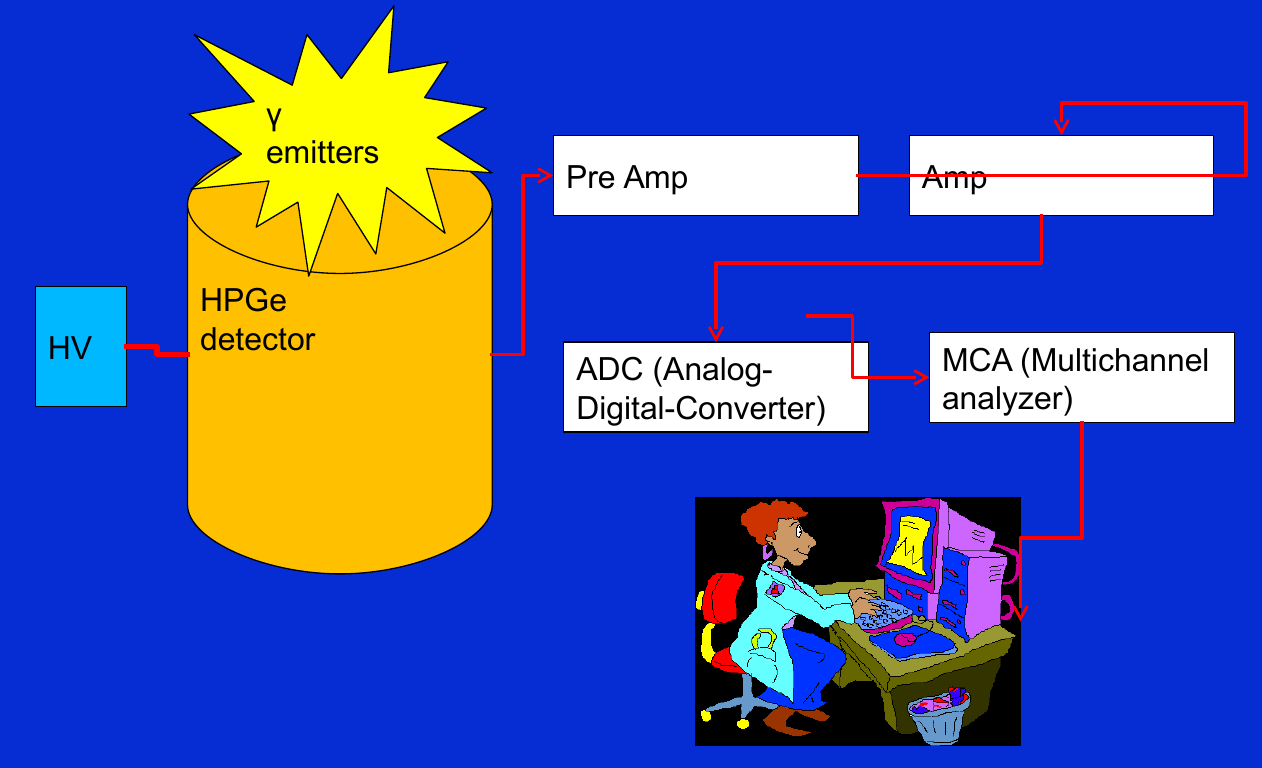
\includegraphics[scale=0.25]{figures/detectionsystem.png}

\end{frame}

\begin{frame}{HPGe detectors}



\begin{itemize}
\item The detector produces a signal proportional to the energy emitted by the source
\item The measuring equipment accumulates on each channel the number of emissions corresponding to a certain energy
\end{itemize}



\pause
\begin{table}
\begin{tabular}{cc}
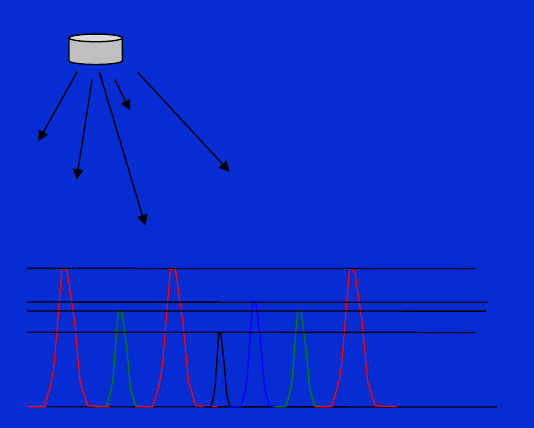
\includegraphics[scale=0.2]{figures/schemedetection1.png} & 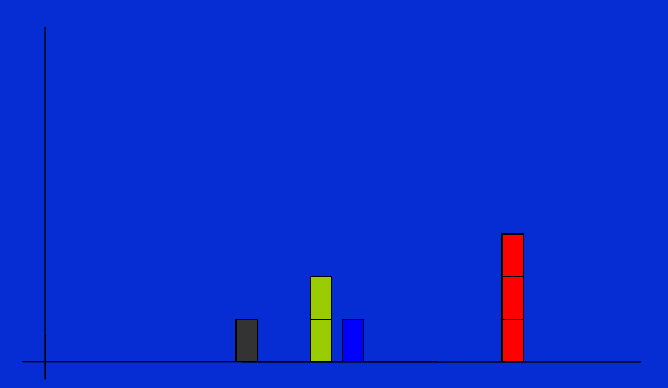
\includegraphics[scale=0.2]{figures/detectionsystem2.png}
\end{tabular}
\end{table}

\end{frame}

\begin{frame}{HPGe detectors: MCA (Multichannel analyzer)}


{\small 
\begin{itemize}
\item From the output from the amplifier, it rejects out-of-range pulses
\item it measures the height of each of those accepted and adds a count into the memory location corresponding to the channel representing the voltage range
\item it displays the data as a spectrum and allows the data to be printed or saved to a data storage device.
\item In principle, the relationship between pulse height (and therefore energy) and channel number would be exactly linear, passing through zero
\end{itemize}
}



\end{frame}

\begin{frame}{HPGe detectors: MCA (Multichannel analyzer)}

\centering
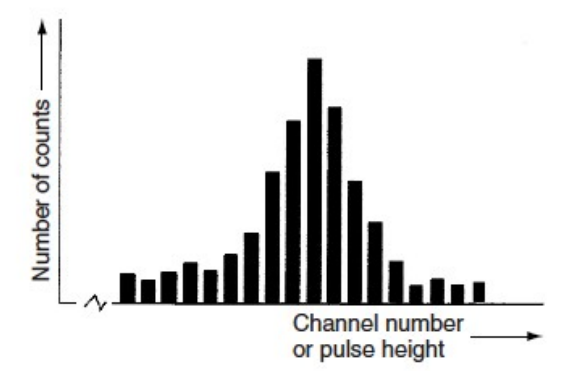
\includegraphics[scale=0.5]{figures/mca.png}

\end{frame}

\begin{frame}{HPGe detectors: MCA terms and definitions}





{\scriptsize 
\begin{itemize}[leftmargin=3.5cm]
\item[Lower level discriminator (LLD)] pulses below this level will not be analysed. Use this to reject electronic noise and low-energy X-rays
\item [Upper level discriminator (ULD)] pulses above this level will not be analysed. Use this to reject very high energy pulses. This will often be left at its maximum, but still performs a useful function in rejecting high- energycosmic gamma-rays
\item [ADC zero level]  use this to adjust the energy calibration so that it passes through 0 keV. Not ideal for eliminating the effect of noise
\item [Digital offset] this is a means of shifting the spectrum to lower channel numbers by subtracting a fixed number (the offset) from every channel number output by the ADC 
\item [Conversion range] the maximum pulse height the MCA can accept, typically 10 V
\item [ADC resolution] is the total number of channels available within the ADC. It varies from model to model, but MCAs for germanium systems might incorporate a 16k (16384), 8k (8192), or 4k (4096) channels ADC
\item [ADC conversion gain] is simply the number of channels actually used in a particular application – in everyday parlance, the spectrum size
\end{itemize}
}




\end{frame}

\begin{frame}{Standards, calibrations}

{\small
\begin{itemize}[leftmargin=3cm]
\item[Geometry] the standard source shall have the same geometry as the sample to be measured. 
\item[Geometry] the standard radioactivy source shall be homogeneously distributed 
\item[Position] centered position
\item[Software] the sorftware determines the presence of isotopes according to their energy. Thermal variations may cause spectrum shifts. Therefore it is necessary to carry out verifications frecuently
\end{itemize}
}

\end{frame}

\begin{frame}{Calibration source}

\begin{table}
\begin{tabular}{m{0.4\textwidth}m{0.4\textwidth}}

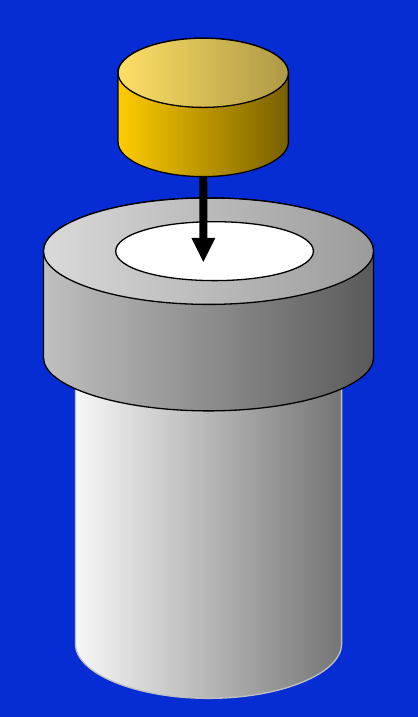
\includegraphics[scale=0.2]{figures/calibration_position.png} & \begin{itemize}
\item Similar density of standard and analysis sample
\item Standard shall be uniformly distributed over the entire volume (similar self-absorption as analysis samples)
\item Centre the sample
\end{itemize}

\end{tabular}
\end{table}

\end{frame}

\begin{frame}{Examples of geometries}

\centering
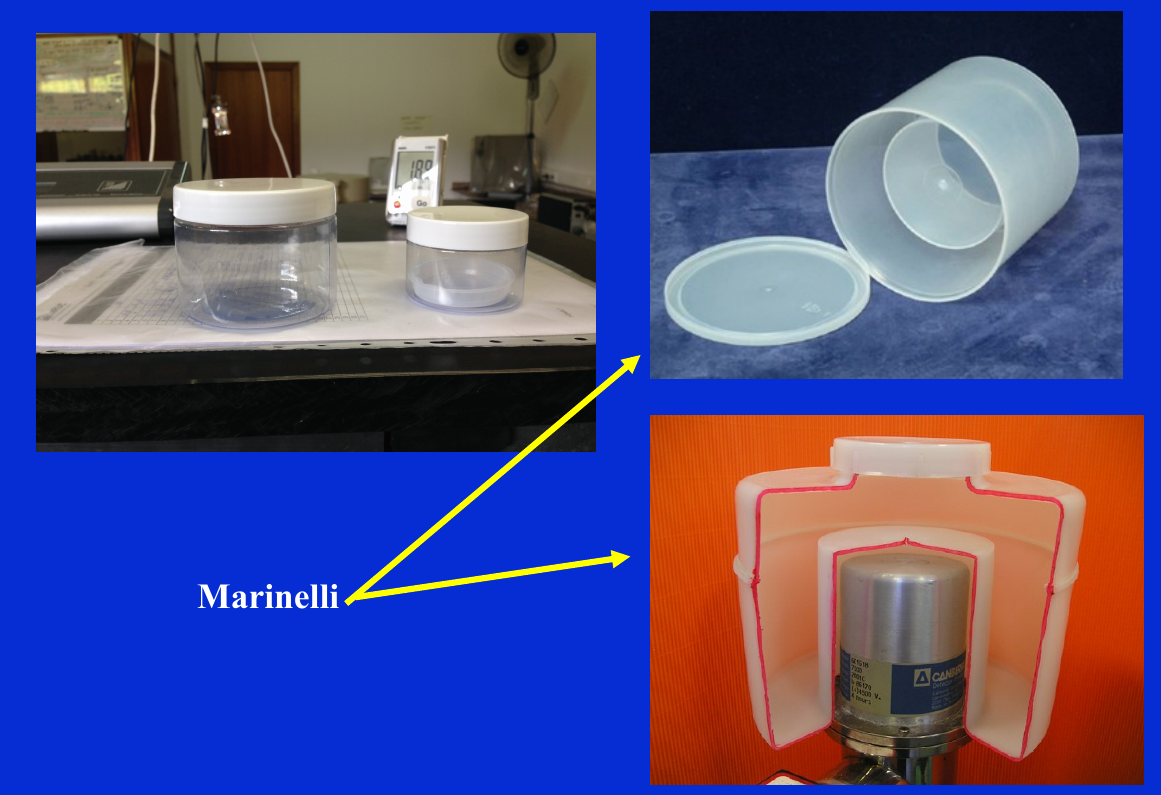
\includegraphics[scale=0.27]{figures/geometries.png}

\end{frame}

\begin{frame}{Calibration steps}

\setbeamercolor{boxsthlmBlue}{bg=\cnBlue,fg=white}\begin{beamercolorbox}[wd=\linewidth,ht=3ex,dp=3ex]{boxsthlmBlue}\centering Calibration energy versus channel  \end{beamercolorbox}


%\vskip5cm
\setbeamercolor{boxsthlmBlue}{bg=\cnBlue,fg=white}\begin{beamercolorbox}[wd=\linewidth,ht=3ex,dp=3ex]{boxsthlmBlue}\centering Calibration efficiency versus enery \end{beamercolorbox}


\end{frame}

\begin{frame}{Energy vs. channel}

\alert{The objective of energy calibration is to derive a relationship between peak position in the spectrum and the corresponding gamma-ray energy}


Energy calibration is accomplished by measuring the spectrum of a source emitting gamma-rays of precisely known energy and comparing the measured peak position with energy. It matters not whether the source contains a single nuclide or several nuclides: $^{152}$Eu source for routine energy calibration


\end{frame}

\begin{frame}{Energy vs. channel}
%\centering
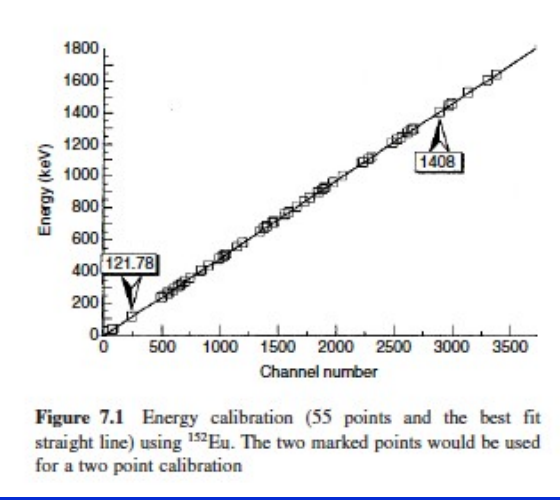
\includegraphics[scale=0.4]{figures/energy_channel.png}
\end{frame}

\begin{frame}{Energy vs. channel}

\centering
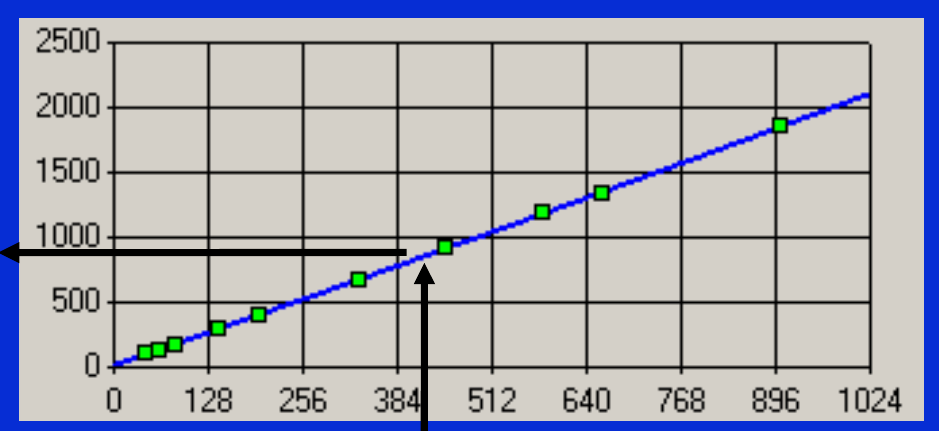
\includegraphics[scale=0.3]{figures/laruc_energy_channel.png}

\end{frame}

\begin{frame}{Efficiency vs. energy}

\begin{flushright}

\begin{minipage}{0.7\textwidth}
{\scriptsize 
\begin{itemize}
\item[Relative efficiency] general performance measure relating the efficiency of detection of the $^{60}$Co gamma ray at 1332 keV of the detector to that of a standard sodium iodide scintillation detector
\item[Absolute full energy peak] relation between the peak area in our spectrum to the amount of radioactivity it represents. This relates the peak area, at a particular energy, to the number of gamma- rays emitted by the source and must depend upon the geometrical arrangement of source and detector
\item[Absolute total efficiency] relates the number of gamma rays emitted by the source to the number of counts detected anywhere in the spectrum. This takes into account the full energy peak and all incomplete absorptions represented by the Compton continuum
\item[Intrinsic efficiency] relates the counts in the spectrum to the number of gamma rays incident on the detector. This efficiency is a basic parameter of the detector and is independent of the source/detector geometry. It is also called full energy peak or total
\end{itemize}
}
\end{minipage}
\end{flushright}

\end{frame}

\begin{frame}{Energy vs. channel}

\centering
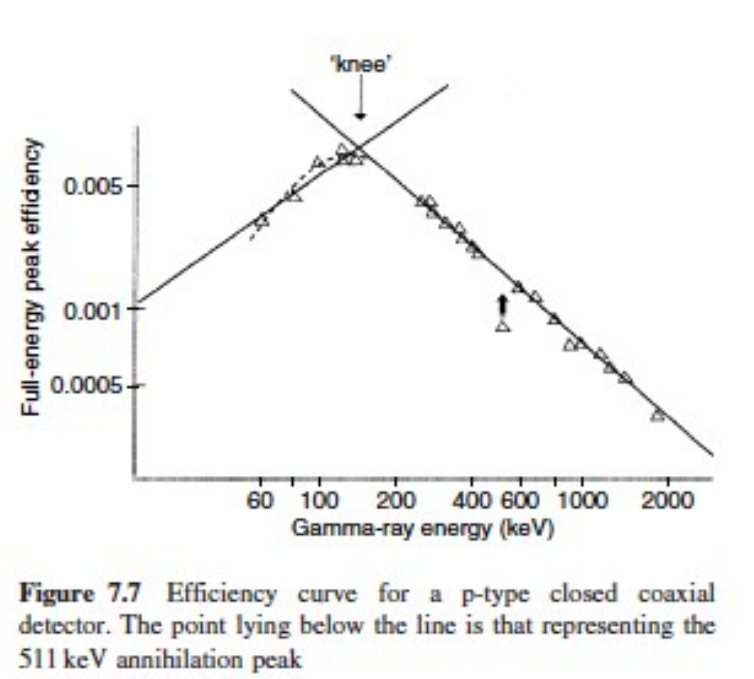
\includegraphics[scale=0.3]{figures/efficiency_energy.png}

\end{frame}

\begin{frame}{Energy vs. channel}

\centering
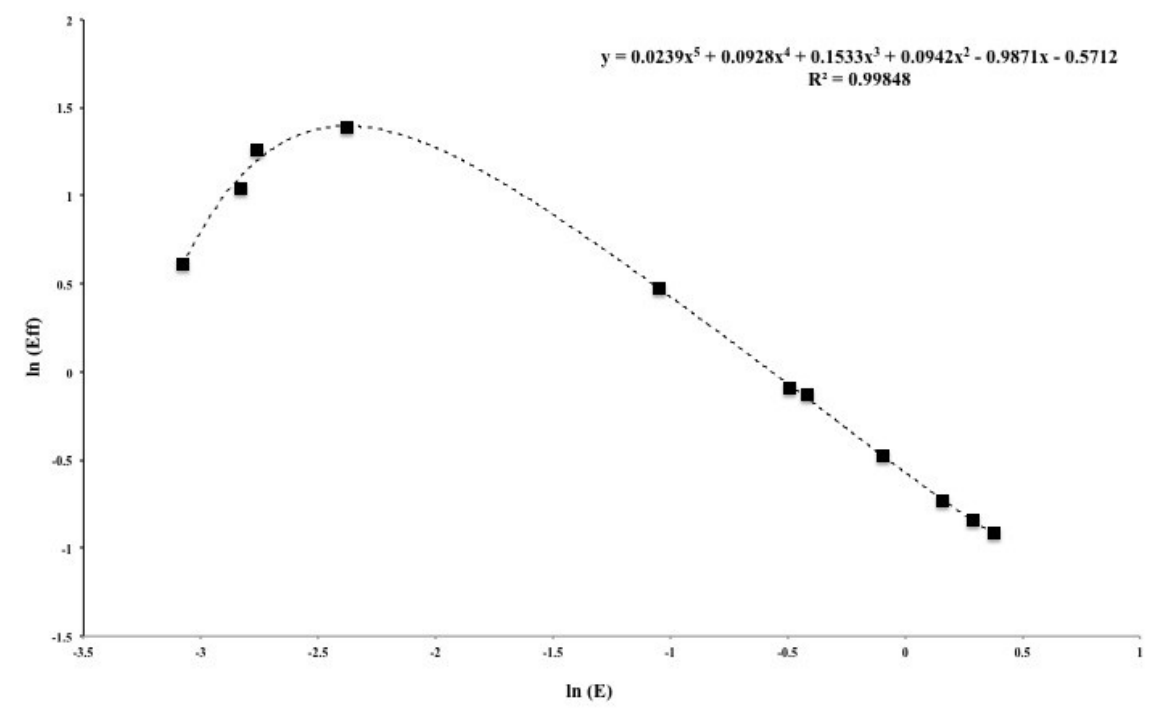
\includegraphics[scale=0.25]{figures/efficiency_energy_laruc.png}

\end{frame}

\begin{frame}{Energy resolution}

\alert{Resolution is a measure of the width of the peaks in a gamma-ray spectrum – the smaller the width, the better the detector, the higher the resolution}

\alert{FHWM: the Full Width of the peak at Half Maximum (keV)}

\centering
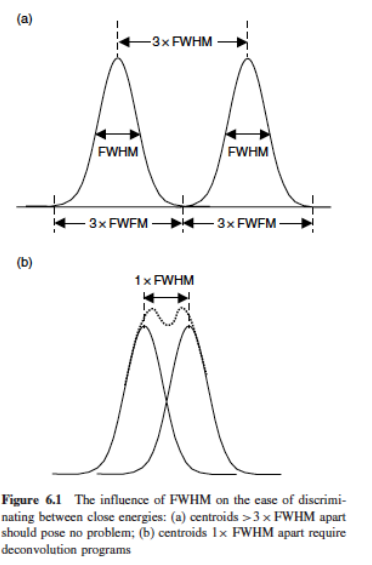
\includegraphics[scale=0.25]{figures/fhwm.png}

\end{frame}

\begin{frame}{Energy resolution}

\centering
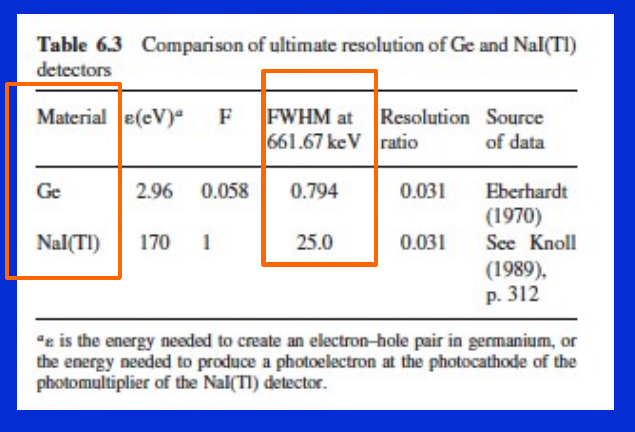
\includegraphics[scale=0.4]{figures/comparisonresolution.png}

\end{frame}

\begin{frame}{How to calculate activity}

\setbeamercolor{boxsthlmBlue}{bg=\cnBlue,fg=white}\begin{beamercolorbox}[wd=\linewidth,ht=3ex,dp=3ex]{boxsthlmBlue}\centering COUNTS\end{beamercolorbox}



\centering \arrowdown

\setbeamercolor{boxsthlmBlue}{bg=\cnBlue,fg=white}\begin{beamercolorbox}[wd=\linewidth,ht=3ex,dp=3ex]{boxsthlmBlue}\centering ACTIVITY (Bq kg$^{-1}$; Bq l$^{-1}$ \ldots)\end{beamercolorbox}


\end{frame}


\begin{frame}{How to calculate activity}


\centering 
\[A = \frac{I}{T\cdot \epsilon \cdot P \cdot X}\]



\begin{itemize}
\item $A$: activity expressed in Bq kg$^{-1}$; Bq l$^{-1}$ \ldots
\item $I$: number of counts corrected
\item $T$: time in seconds
\item $\epsilon$: efficiency
\item $P$: emission probability
\item $X$: mass (kg), volume (l), \ldots
\end{itemize}

In some cases it is necessary to include corrections due to radioactivity decay, summing effects, etc.



\end{frame}

\begin{frame}{Some statistics}

{\centering \alert{Binomial distribution}}

In principle, the statistics of radioactive decay are binomial in nature. If we were to toss a handful of coins onto a table and then examine the arrangement, we would find coins in one of two dispositions – heads up or tails up. Similarly, if we could prepare a radioactive source and, during a particular period of time, monitor each individual atom we would see that each has only one of two possible fates – to decay or not decay

\end{frame}

\begin{frame}{Some statistics}

{\centering \alert{Confidence limits}}

\emph{\ldots we must quote our limits in such a way that we have a stated degree of confidence that the true value lies somewhere within them}

\centering
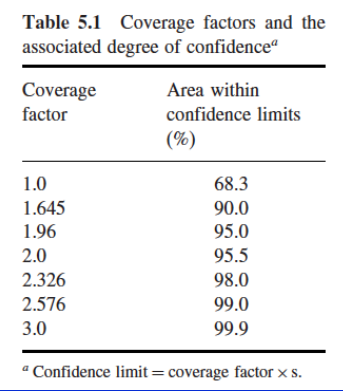
\includegraphics[scale=0.4]{figures/confidencelimits.png}

\end{frame}

\begin{frame}{Some statistics}

\alert{Counting Decision Limits}

\begin{flushright}

\begin{minipage}{0.6\textwidth}
{\scriptsize 
\begin{itemize}
\item[Critical limit (LC)] a decision level: ‘Is the net count significant?’
\item[Upper limit (LU)] ‘Given that this count is not statistically significant, what is the maximum statistically reasonable count?’
\item[Detection limit (LD)] ‘What is the minimum number of counts I can be confident of detecting?’
\item[Determination limit (LQ)] ‘How many counts would I have to have to achieve a particular statistical uncertainty?’
\item[Minimum detectable activity (MDA)] ‘What is the least amount of activity I can be confident of detecting?’
\end{itemize}
}
\end{minipage}
\end{flushright}

\end{frame}

\begin{frame}{Learnings so far}

\begin{alertblock}{Let's remember}

\begin{itemize}

\pause \item Techniques to measure radioactivity: alpha, beta, gamma spectrometry and LSC and gross alpha/beta

\pause \item Interaction of radiation with matter

\pause \item Gamma spectrometry: fundamentals, essential set up procedures

\pause \item Characteristics of HPGe detectors

\pause \item Elementary estatistics of radioactivity


\end{itemize}

\end{alertblock}

\end{frame}